\documentclass[a4paper,12pt]{article}
%\usepackage{fullpage}
%\usepackage{pdfpages}

\usepackage{geometry}
 \geometry{
 a4paper,
 total={170mm,257mm},
 left=20mm,
 top=20mm,
 }

\usepackage{color}
\usepackage{amsmath,graphicx,makeidx}
\usepackage{lscape}
\usepackage{fancyhdr}
\addtolength{\headheight}{1.5cm} % make more space for the header
\pagestyle{fancyplain} % use fancy for all pages except chapter start
\lhead{
\includegraphics[height=1.7cm]{FOSSEE-logo}} % left logo
\rhead{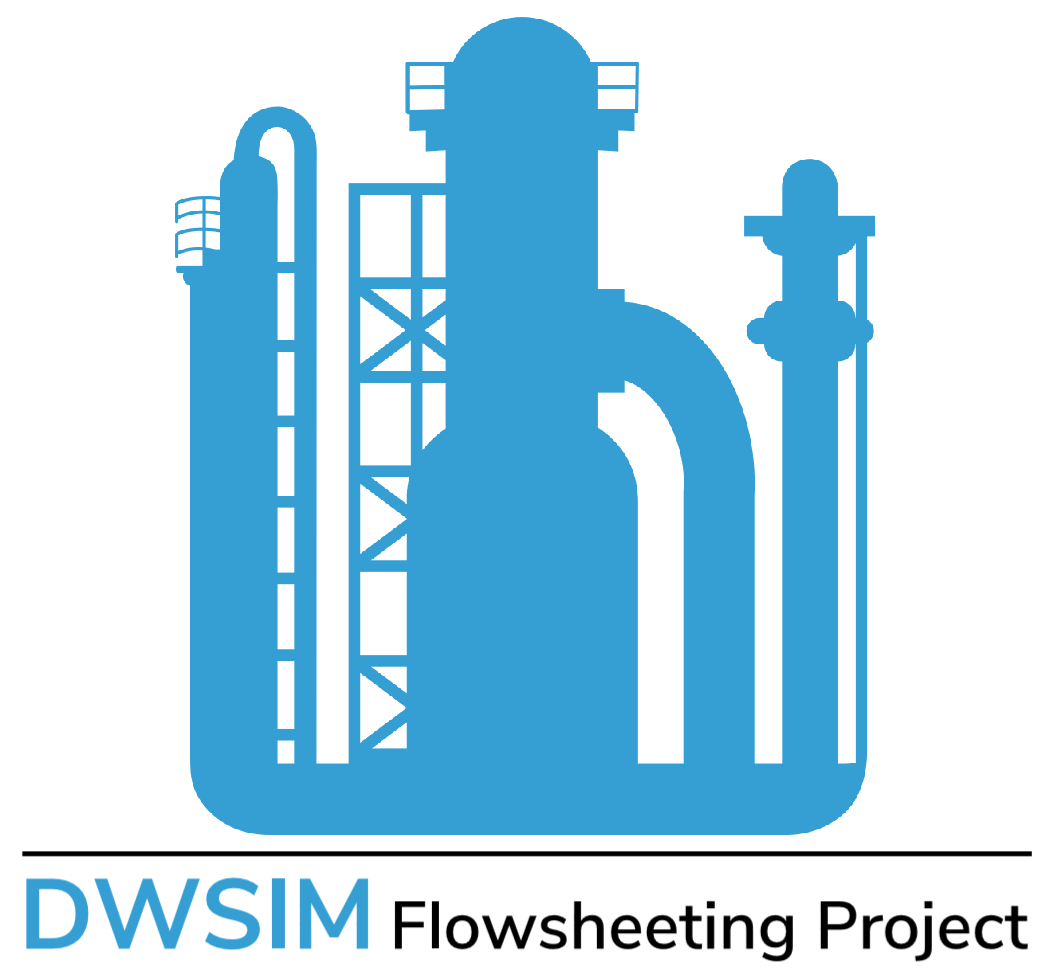
\includegraphics[height=3.5cm]{DWSIM-flowsheeting-project-logo}} % right logo
\renewcommand{\headrulewidth}{0pt} % remove rule below header

\title{Nitrogen Liquefaction using Linde Cycle} %Title of the flowsheet
\author{Priyam Nayak \\ Indian Institute of Technology Bombay} %Institute Name
\date{}


\begin{document}

\maketitle

\noindent \textbf{Background \& Description:} \newline A process for gas liquefaction, particularly nitrogen liquefaction, which combines the use of a nitrogen auto-refrigeration cooling cycle with one or more closed-loop refrigeration cycles using two or more refrigerant components. The closed-loop refrigeration cycle provide refrigeration in a temperature range having a lowest temperature between about -125$^\circ$F. and about -250$^\circ$F. A nitrogen expander cycle provides additional refrigeration, a portion of which is provided at temperatures below the lowest temperature of the closed-loop or recirculating refrigeration cycle or cycles. The lowest temperature of the nitrogen expander cycle refrigeration range is between about -220$^\circ$F. and about -320$^\circ$F. The combined use of the two different refrigerant systems allows each system to operate most efficiently in the optimum temperature range, thereby reducing the power consumption required for liquefaction.

Gaseous nitrogen at 80$^\circ$F, 1 atm is compressed to 25 atm pressure. Adiabatic compressor is employed for this purpose with 50\% efficiency which also results in increasing the temperature of $N_2$ stream to 1577$^\circ$F. The stream is further cooled to -306$^\circ$F with the help of a series of cooler and heat exchanger. Cooled $N_2$ is further expanded by reducing the pressure to 1 atm using an isenthalpic valve to obtain liquefied $N_2$.

\vspace{15mm}
\centerline{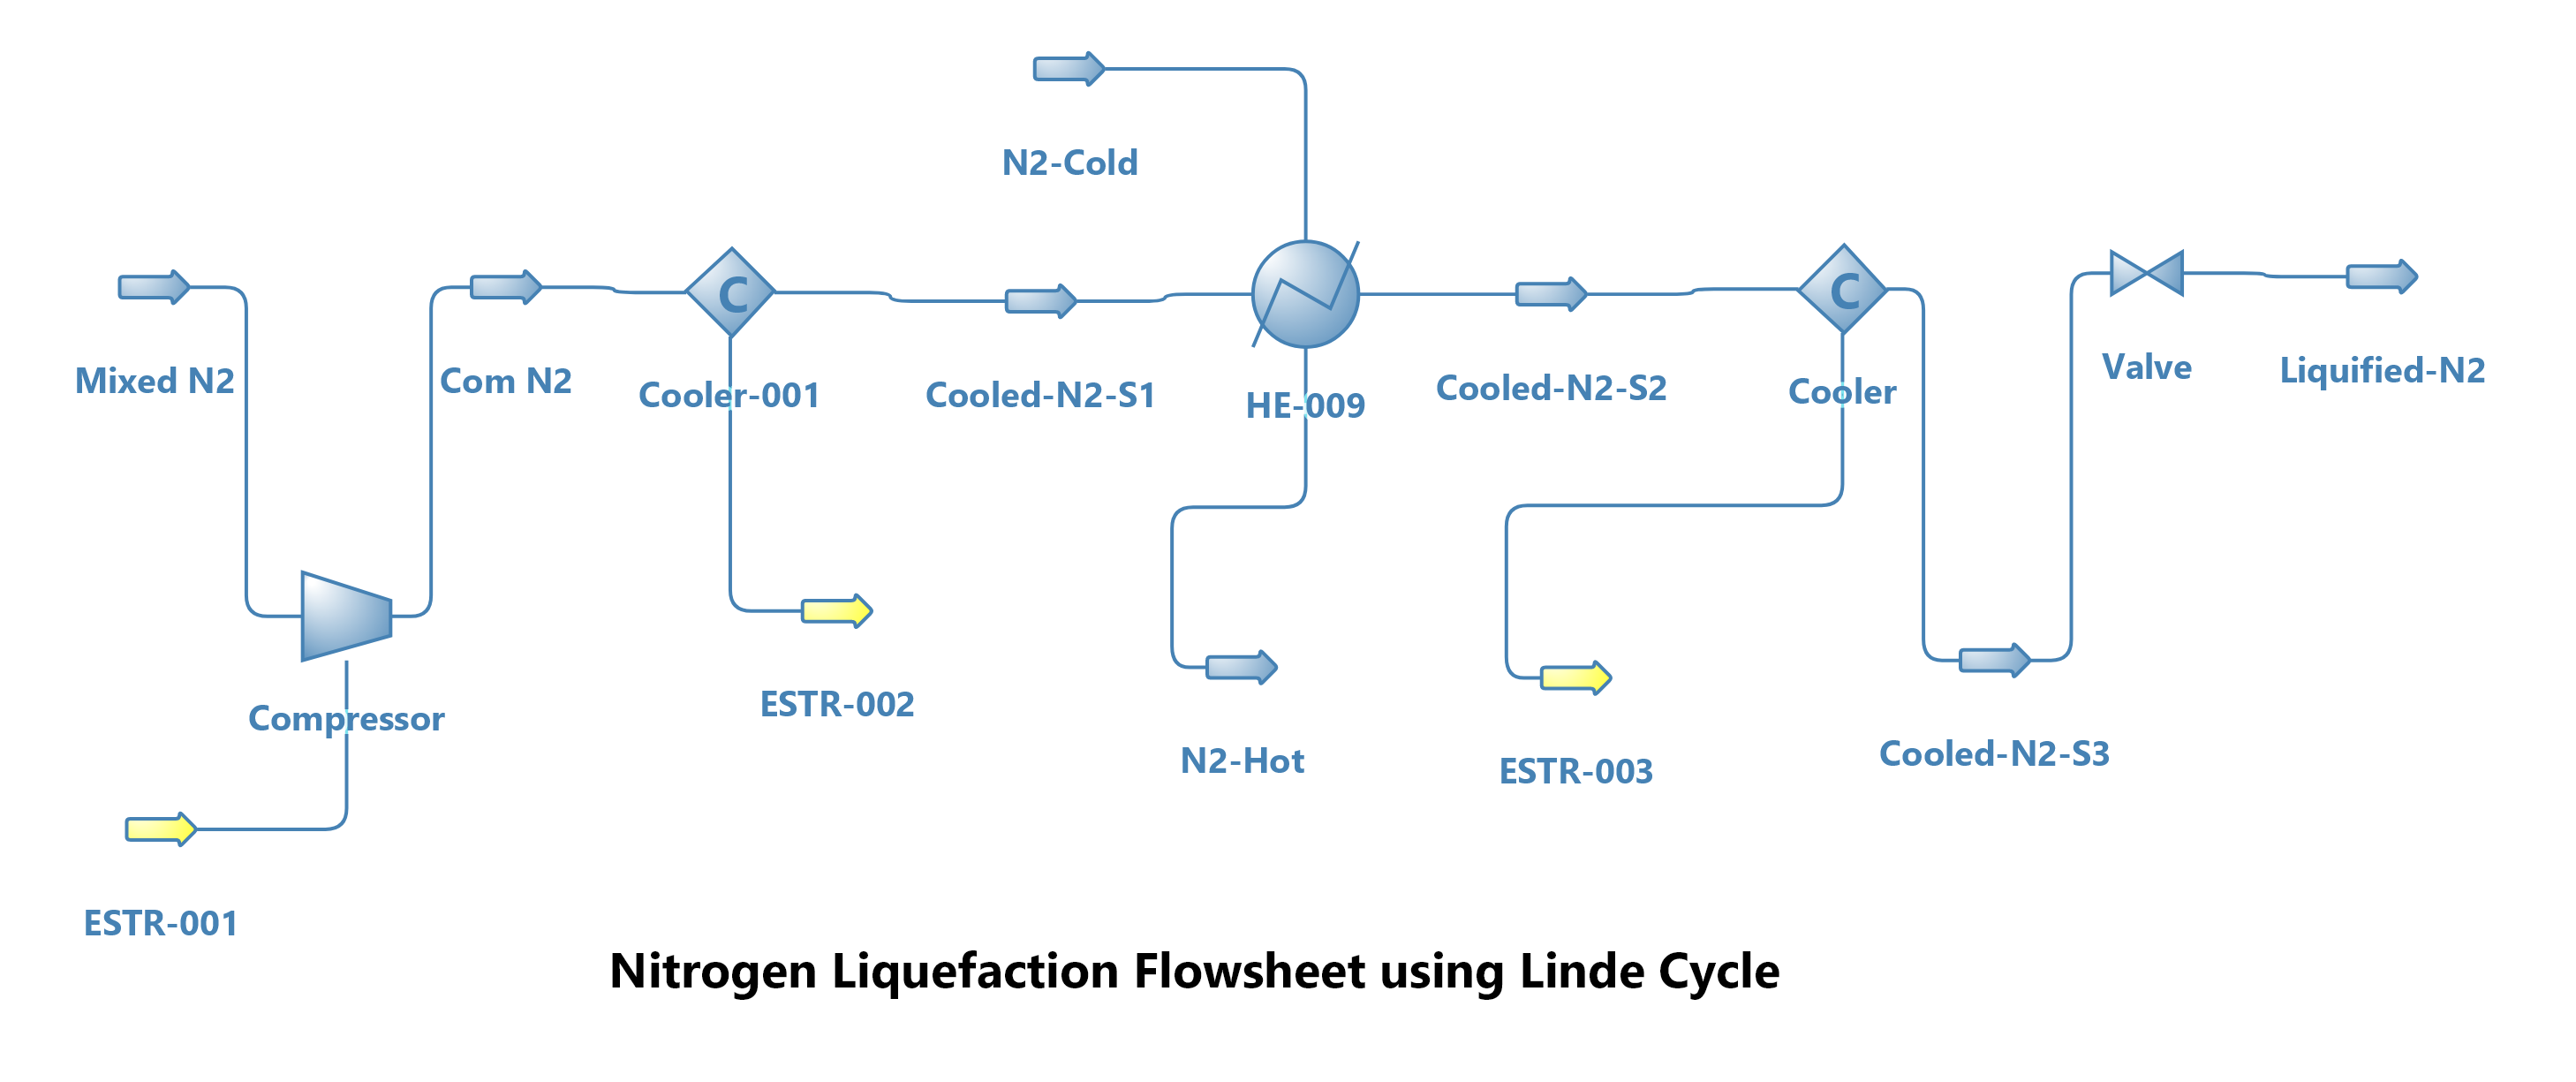
\includegraphics[width=1.2\linewidth]{N2-Liq.png}}

\newpage
\noindent \textbf{Results:}
\begin{table}[h]
%\centering
\resizebox{\textwidth}{!}{%
\begin{tabular}{|l|l|l|l|l|l|}
\hline
\bf Object                                & N2-Hot        & N2-Cold       & Mixed N2      & Liquified-N2 &         \\ \hline
Temperature                           & 229.000009    & 77.354723     & 300.000000    & 77.354722     & K       \\ \hline
Pressure                              & 1.000000      & 1.000000      & 1.000000      & 1.000000      & atm     \\ \hline
Mass Flow                             & 810.000000    & 810.000000    & 1,000.000000  & 1,000.000000  & kg/h    \\ \hline
Molar low                            & 28.914114     & 28.914114     & 35.696437     & 35.696437     & kmol/h  \\ \hline
Volumetric Flow                       & 9,039.506245  & 2,933.487221  & 14,638.558044 & 317.457296    & L/min   \\ \hline
Vapor Phase Molar Enthalpy            & -2,026.180673 & -6,491.084701 & 46.205128     & -6,491.084717 & kJ/kmol \\ \hline
Mass Flow (Vapor Phase) / Nitrogen    & 810.000000    & 810.000000    & 1,000.000000  & 82.385093     & kg/h    \\ \hline
Mass Flow (Liquid Phase 1) / Nitrogen & 0.000000      & 0.000000      & 0.000000      & 917.614907    & kg/h    \\ \hline \hline
\bf Object                                & Cooled-N2-S3  & Cooled-N2-S2  & Cooled-N2-S1  & Com N2        &         \\ \hline
Temperature                           & 85.000000     & 185.421934    & 300.000000    & 1,131.982017  & K       \\ \hline
Pressure                              & 25.000000     & 25.000000     & 25.000000     & 25.000000     & atm     \\ \hline
Mass Flow                             & 1,000.000000  & 1,000.000000  & 1,000.000000  & 1,000.000000  & kg/h    \\ \hline
Molar Flow                            & 35.696437     & 35.696437     & 35.696437     & 35.696437     & kmol/h  \\ \hline
Volumetric Flow                       & 21.548744     & 330.795696    & 580.618715    & 2,224.492556  & L/min   \\ \hline
Vapor Phase Molar Enthalpy            & 0.000000      & -3,747.282874 & -130.711665   & 25,876.051649 & kJ/kmol \\ \hline
Mass Flow (Vapor Phase) / Nitrogen    & 0.000000      & 1,000.000000  & 1,000.000000  & 1,000.000000  & kg/h    \\ \hline
Mass Flow (Liquid Phase 1) / Nitrogen & 1,000.000000  & 0.000000      & 0.000000      & 0.000000      & kg/h    \\ \hline
\end{tabular}%
}
\caption{Streamwise Results for the Nitrogen Liquefaction Flowsheet}
\end{table}


\end{document}


